\documentclass{article} % For LaTeX2e
\usepackage{nips15submit_e,times}
\usepackage{hyperref}
\usepackage{url}
\usepackage{graphicx}
%\documentstyle[nips14submit_09,times,art10]{article} % For LaTeX 2.09

\title{Machine Learning Project}

\author{
Alex Brinkman\\
Robotics Institute\\
Carnegie Mellon University\\
Pittsburgh, PA 15213 \\
\texttt{abrinkma@andrew.cmu.edu} \\
\And
Abhishek Bhatia \\
Robotics Institute \\
Carnegie Mellon University\\
Pittsburgh, PA 15213 \\
\texttt{abhatia1@andrew.cmu.edu} \\
}

\newcommand{\fix}{\marginpar{FIX}}
\newcommand{\new}{\marginpar{NEW}}

\nipsfinalcopy % Uncomment for camera-ready version

\begin{document}

\maketitle

\begin{abstract}
abstract goes here TODO

\end{abstract}

\section{Part 1}
The goal of the project for part 1 is to classify subject behavior baed on raw voxel activation values.  The final approach developed to achieve this goal includes an SVM classifier, custom feature extraction, and a voting method. The resulting accuracy was 60.47\% on the holdout data set.

\subsection{SVM Classifier}
Abhishek

\subsection{Custom Feature Extraction}
The custom feature extraction....

\begin{figure}[H]
\begin{center}
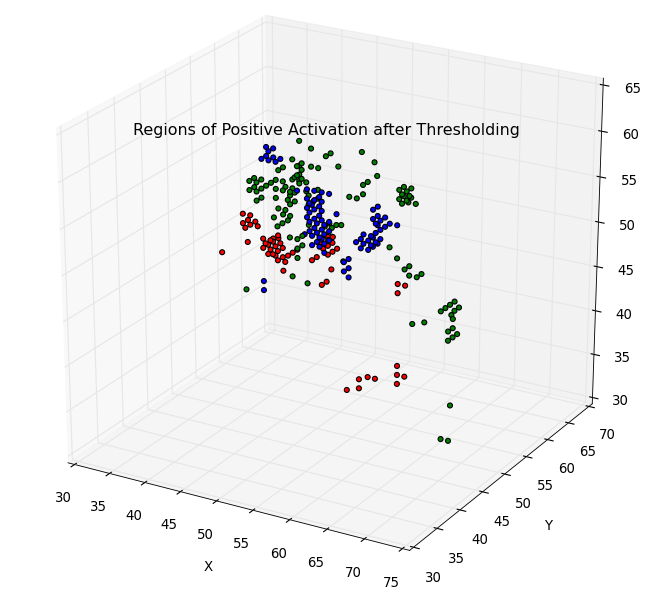
\includegraphics[scale=.4]{media/pos_activation_formatted.png}
\end{center}
\caption{Sample figure caption.}
\end{figure}



\begin{table}[H]
\caption{Sample table title}
\label{sample-table}
\begin{center}
\begin{tabular}{ll}
\multicolumn{1}{c}{\bf HEADING C1}  &\multicolumn{1}{c}{\bf HEADING C2}
\\ \hline \\
r1c1   &r1c2       \\
r2c1   &r2c2 \\
etc		&etc\\
\end{tabular}
\end{center}
\end{table}

\subsection{Voting Method}

\section{Part 2}
\subsection{Ridge and Lasso Classifiers}
\subsection{MultiTaskLasso Cross Validation}

MultiTask Lasso begin


\begin{figure}[H]
\begin{center}
%\framebox[4.0in]{$\;$}
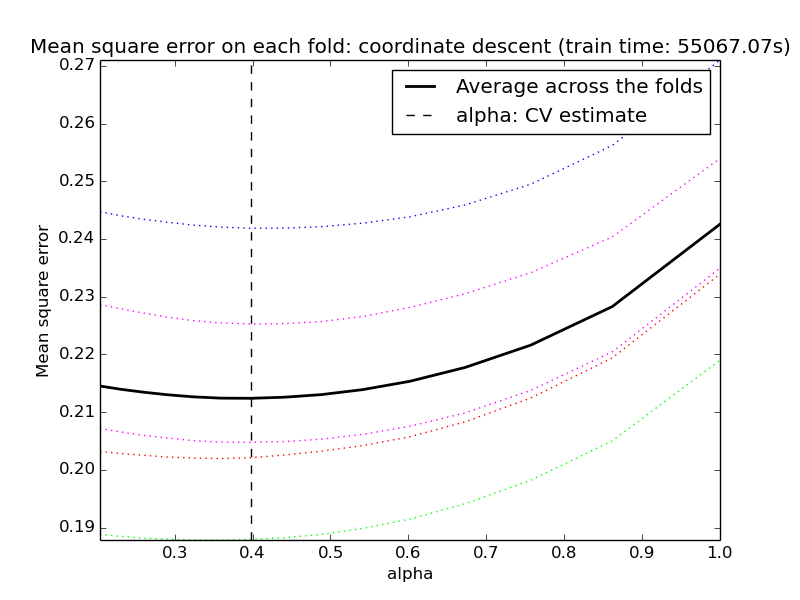
\includegraphics[scale=.5]{media/cross_validation_figure_2.png}
\end{center}
\caption{Sample figure caption.}
\end{figure}

multitask lasso end

\subsection{Euclidean Clustering}


\section{Part 3}

\subsection{Hypothesis}

\subsection{Experiment}

\subsection{Results}




\subsubsection*{References}

\small{
[1] Scikit-learn: Machine Learning in Python, Pedregosa et al., JMLR 12, pp. 2825-2830, 2011.
}

\end{document}
